\chapter{Interface graphique}\label{chap:GUI}
    \section{Le jeu}
        \subsection{La fenêtre de Jeu}
            \paragraph{}C'est un élément déterminant car il est ce que voit l'utilisateur est c'est par celui-ci est uniquement celui-ci que le programme communique avec ce dernier. Bien que central cet élément \textbf{ne gère pas les choses lui-même}, en effet il se contente de \textbf{communiquer les événements qu'il reçoit} à ses composantes que sont le \textit{Plateau (le Goban)} et \textit{la zone d'infos.}
            
            \paragraph{}La fenêtre de jeu fait donc principalement office \textbf{d'interface} et sa fonction se résume à savoir qui des \textit{infos} ou du \textit{plateau} est apte à \textit{traiter l'information} reçue. C'est donc un des éléments situés au plus \textbf{haut niveau} avec les différents menus, cette catégorie d'objet est celle ayant en charge la \textbf{boucle principale} et s'affichant directement à l'écran.
            
            \begin{figure}[h!]
            \centering
            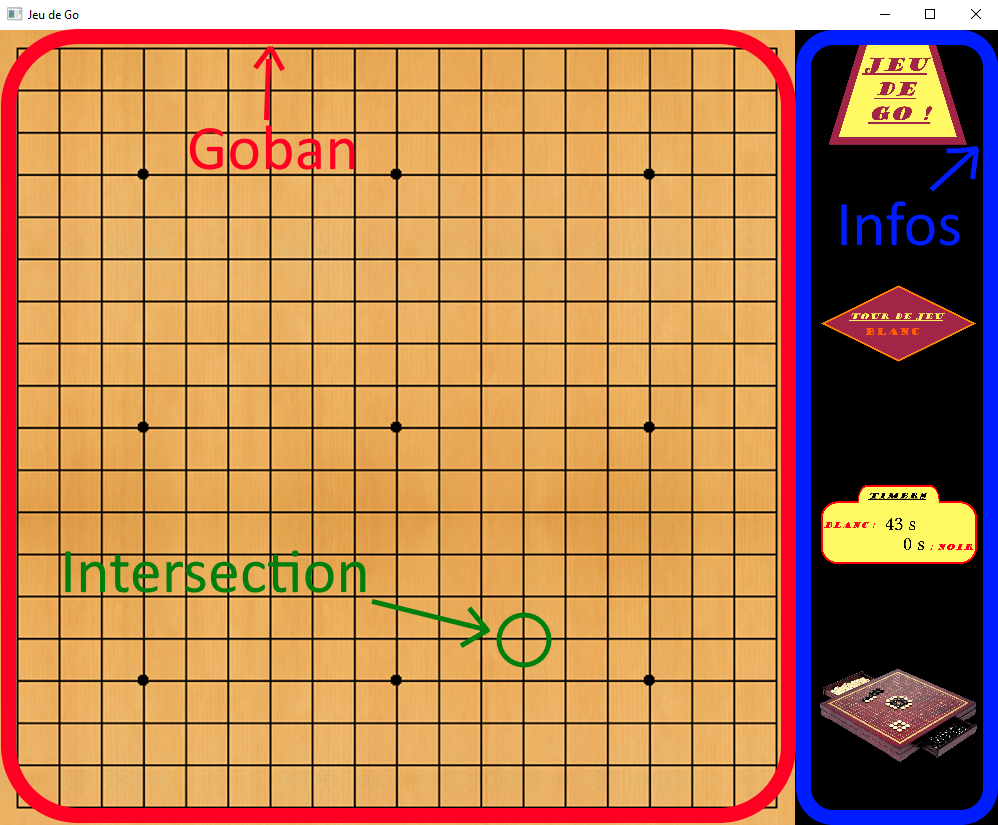
\includegraphics[scale=0.45]{figures/experiments/Fenetre_de_jeu.png}
            \caption{Fenêtre de Jeu}
            \label{fig:game}
            \end{figure}
            
        \subsection{Une partie de Go}
            \paragraph{}Le goban est composé tout d'abord d'un \textbf{visuel} -son apparence- qui peut éventuellement changer selon les goûts de l'utilisateur. On peut aussi souhaiter se concentrer simplement sur une partie du plateau et pour cela il convient d'autoriser un \textbf{zoom} afin de correspondre au mieux à la zone pertinente aux yeux de l'utilisateur.   
            
        	\paragraph{}De plus le plateau est l'élément qui \textbf{interface} avec le \textit{'moteur'} du jeu, c’est à dire les différentes \textit{règles du jeu}. Pour cela il convient de lui permettre de faire la jonction correctement entre le visuel -qui est destiné à l'utilisateur- et ce moteur. Évidemment ceci fonctionne dans les deux sens et \textbf{les actions utilisateur} (clavier, souris, ...) doivent être interceptées par cet élément pour \textbf{être transmises} aux \textit{règles} qui lui dicteront en retour l'action à entreprendre (par exemple pour un feed-back).
        	
        	\paragraph{}Bien qu'il fasse office de passerelle avec le moteur, il convient de ne pas résumer le goban simplement à cette fonction munie d'un visuel. En effet le goban représente avant tout \textbf{la zone de jeu} et celle-ci est composé d'un élément capital : \textit{les intersections} où sont posées les pierres.
        	
    	\subsection{L'intersection}
    	    \paragraph{}Dans un goban l'intersection joue un rôle majeur et chacune d'entre elles possède diverses informations qu'il est nécessaire de bien définir afin de pouvoir les représenter. \\
        	Parmi ces informations on distingue deux types d'information : celles \textbf{propres à chaque intersection} et celles \textbf{communes à toutes les intersections}.      
        	
        	\paragraph{}Pour ce qui est des informations communes, on trouve simplement \textbf{l'apparence des pierres}. Celle-ci doit en effet être la même indépendamment de l'intersection où se trouve la pierre. D'autres informations pourraient être relevées mais elles n'ont pas d'implication dans notre application. C'est notamment le cas du poids des pierres, de leur animation de pose / de prise, de leurs sons dans divers cas, etc...        	
        	
        	\paragraph{}Concernant les informations distinctes, celles-ci sont un peu plus nombreuses. Il faut retenir -entre autres- \textbf{la position} de chaque intersection ainsi que \textbf{sa 'valeur'} (i.e. si c'est une pierre noire, blanche ou s'il n'y a pas de pierre du tout). Pas d'autre information effectivement utilisée n'est à relever ici.
        	
	    \subsection{La zone d'infos}
	        \paragraph{}Si une partie de Go pourrait se résumer à un \textit{plateau et des pierres}, certaines informations manquent cruellement à cette définition. C'est notamment le cas du \textbf{joueur actuel} car le jeu de Go se joue au tour par tour comme la très grande majorité des jeux de plateau. Mais aussi du \textbf{temps passé} par chaque joueur depuis le début de la partie. En effet certaines règles imposent un temps de jeu limité par coup / global ; et lorsque ce n'est pas imposé, il est tout de même souhaitable de disposer visuellement de ces informations.
	         
	         
    \section{Les menus}
        \subsection{Définition des menus}
            \paragraph{}Lorsque l’on développe une \textbf{application graphique} il arrive un moment où il convient d’intégrer un menu à celle-ci afin de la rendre \textbf{navigable et configurable} par l’utilisateur. Malheureusement cette partie peut s’avérer très longue et fastidieuse avant d’arriver à un résultat convenable. Aussi il faut bien souvent choisir entre des menus lourds très personnalisables mais longs à intégrer et des menus plus génériques mais intégrables rapidement. Nous avons opté pour cette seconde méthode qui –bien qu’elle soit plus longue à préparer- permet de \textbf{rajouter facilement des menus, des items, etc…} Nous allons détailler ici les menus génériques tels qui \textit{peuvent être intégrés} à n’importe quel autre programme.
            
            \begin{figure}[h!]
            \centering
            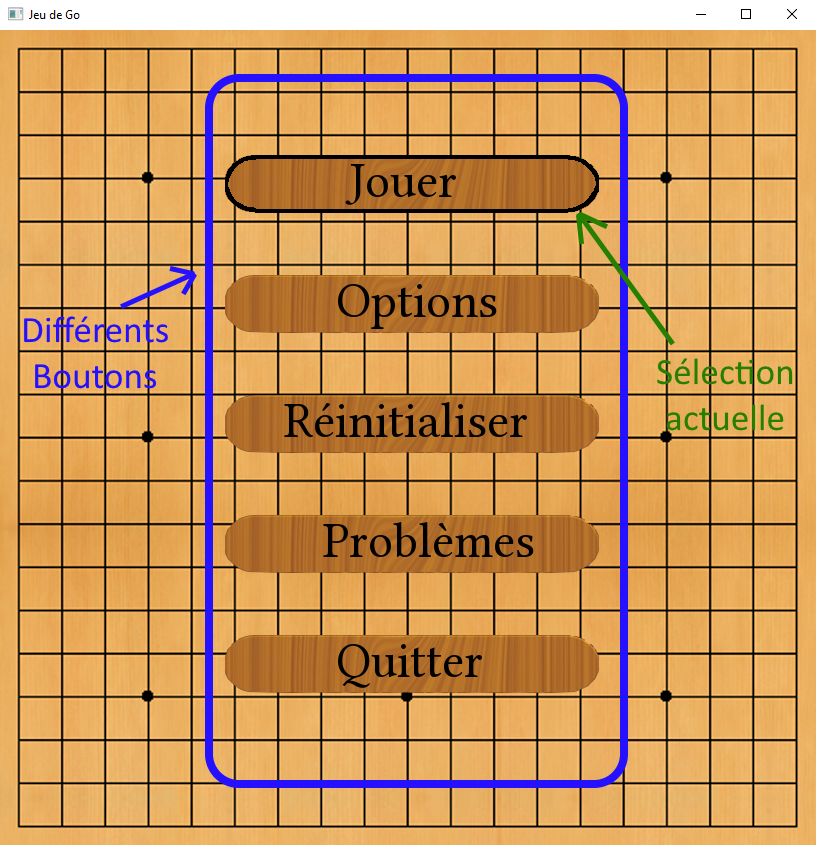
\includegraphics[scale=0.45]{figures/experiments/Menu_main.png}
            \caption{Menu où les boutons ont la même texture mais un texte différent}
            \label{fig:butto_txt}
            \end{figure}
            
	        \paragraph{}Pour cela nous devons identifier ce qu’est un menu et ce qu’il permet de réaliser. Tout d’abord un menu est un \textbf{élément visuel navigable} qui permet à \textit{l’utilisateur} \textbf{d’interagir} avec le programme. Chaque menu est donc composé d’éléments visuels tels que \textbf{l’arrière-plan}. De plus chaque menu possède différents \textit{boutons}. Comme dit ci-dessus les menus doivent être capables d’interagir avec l’utilisateur, notamment un menu doit permettre de \textbf{naviguer} librement entre les différents \textit{choix} qu’il propose ainsi que de mettre en valeur le \textit{choix actuellement sélectionné} par l’utilisateur. En plus de pouvoir naviguer parmi différents choix, l’utilisateur peut souhaiter aussi pouvoir \textbf{valider} le choix actuellement sélectionné, il faut donc lui en donner l’opportunité. 
	        
            \paragraph{}Une fois que ces principes de bases sont posés on peut réfléchir à la façon dont les menus doivent être créés par le programmeur. Pour créer un menu il faut donc \textbf{une position}, éventuellement \textbf{ menu précédent} et \textbf{un aspect} (l’arrière-plan). Le menu ne se suffisant pas à lui-même il faut permettre \textbf{l’ajout \textit{d’items}} en son sein. Nous nous sommes arrêté ici car ces menus doivent répondre à des besoins basiques notre projet étant en temps limité.
             
        \subsection{Définition des items}
            \paragraph{}Comme \textit{un menu} ne peut se passer de boutons nous avons créé ceux-ci et, là aussi, un peu de réflexion a été de mise. Tout comme les menus, les boutons possèdent \textbf{un aspect}. En fait ils en possèdent même plusieurs selon \textbf{leur état}.
            \paragraph{}En effet les boutons possèdent différents états qui peuvent parfois se \textbf{cumuler}. Notamment ils peuvent être \textbf{sélectionnés}, \textbf{survolés} par la souris, \textbf{enfoncés} par un click, voir ne pas avoir d’état particulier, un peu à la manière des \textit{liens HTML}.
            
            \begin{figure}[h!]
            \centering
            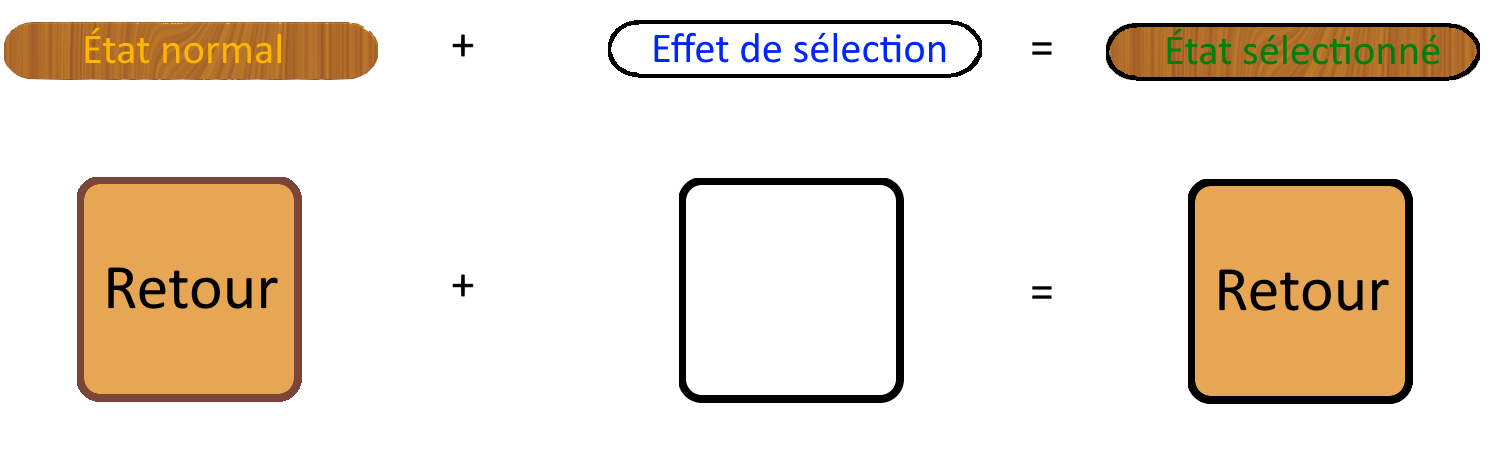
\includegraphics[scale=0.30]{figures/experiments/Effet_Select.png}
            \caption{Application d'effets aux boutons}
            \label{fig:button}
            \end{figure}
            
            \paragraph{}Ces états déterminent donc \textbf{l’affichage du bouton} et c’est pourquoi celui-ci possède \textit{plusieurs aspects} même si un seul est affiché à la fois. Le bouton doit contenir en permanence son \textbf{état actuel} qui sera changé par le \textit{menu auquel il appartient}. Enfin pour en finir avec l’aspect des boutons ceux-ci possèdent bien évidement \textbf{une position} relative au menu auquel ils appartiennent ainsi qu’\textbf{une zone de collision} permettant au \textit{menu} de déterminer si l’utilisateur pointe sa souris sur tel ou tel bouton.
            
            \paragraph{}Enfin les boutons ne sont pas juste là pour décorer et leur fonction principale est de permettre \textbf{d’effectuer une action} lors de la sélection de ceux-ci. Une fois \textit{validé} un bouton peut permettre des actions aussi \textit{diverses} que couper la musique revenir au menu précédent, lancer une partie de Go ou même quitter le jeu.

        \subsection{Les cas spéciaux}
            \paragraph{}Une fois les menus et boutons créés nous nous sommes rendu compte en les utilisant -pour créer les différents menus du jeu- que certaines tâches répétitives persistaient et que les menus pouvaient donc encore être améliorés. 
            
            \begin{figure}[h!]
            \centering
            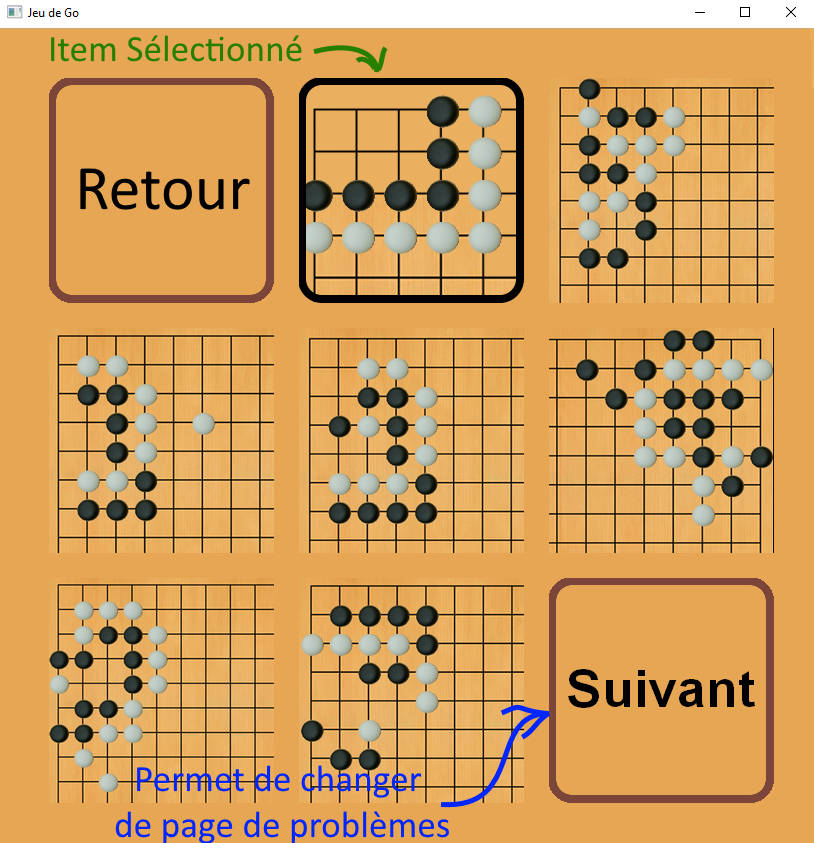
\includegraphics[scale=0.45]{figures/experiments/Menu_pbs.png}
            \caption{Menu où chaque bouton a sa propre texture}
            \label{fig:menu_prbls}
            \end{figure}
            
            \paragraph{}Par exemple dans le cas où \textit{sélectionner un item} ne doit \textbf{pas changer son apparence} mais simplement lui appliquer une \textbf{mise en valeur} (par exemple un lisserait noir l’entourant dans notre cas). Pour régler ceci et afin \textbf{d’alléger la mémoire} dans ce genre de cas de figure assez courant nous avons choisi de dériver notre objet menu en une variante contenant -en plus de tout ce que possède déjà un menu- \textbf{l’effet à appliquer} au bouton sélectionné. 
             
            \paragraph{}Nous avons aussi fait le choix de dériver à nouveau notre menu pour lui ajouter une autre fonctionnalité : \textbf{le texte}. En effet nous souhaitions créer des \textbf{boutons avec un texte} et nous n’avions besoin que d’une \textbf{police de caractère} pour tous les boutons du menu –nul besoin d’alourdir la mémoire avec la même police chargé X fois en mémoire là où une suffirait.
            Pour aller avec ces deux nouveaux menus nous avons de la même manière dérivé les boutons pour qu’ils puissent contenir soit leur \textit{propre texture} pour le $1^{er}$ cas soit \textit{leur texte} pour le $2^{nd}$ cas.
            
            \paragraph{}Tout ceci permet dans cette application un léger \textbf{gain mémoire} (dans notre exemple celui-ci est de d’un facteur 50) qui, dans le cas d’une application plus volumineuse avec de nombreux menus et surtout des ressources plus gourmandes en mémoires, permet d’atteindre des gains bien plus conséquent.
            
            \begin{figure}[h!]
            \centering
            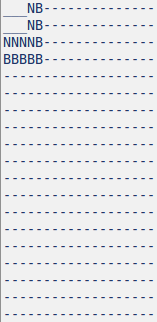
\includegraphics[scale=0.39]{figures/experiments/fichierGo.png}
            \caption{Le fichier .go du problème du 6 en coin}
            \label{fig:menu_prbls}
            \end{figure}

    \section{Les ressources}
        \subsection{La musique}
            \paragraph{}La musique a été réalisé à l'aide du logiciel "full studio 10 ". Elle essaie de traduire le plus possible l'univers du Go. Un univers asiatique et combatif.\\
            Les bandes de sons concernant la prise d'un groupe et la pose d'une pierre ont été téléchargé sur un site de banque de son gratuit. Étant, l'un le bruit d'une explosion et l'autre le bruit d'un marteau sur du bois, ils ont été modifié et traité afin de mieux correspondre à nos besoins.
    
        \subsection{Les images}
            \paragraph{} images quant à elles proviennent de diverses sources, pour la plupart elles ont été traités (détourage, filtres) avant d'être utilisés dans l'interface, certaines ont aussi été créés directement comme par exemple pour les menus.